\باب{لاپلاس تبادلہ}
لاپلاس بدل کی ترکیب سے ابتدائی قیمت (سرحدی قیمت) تفرقی مساوات حل کیے جاتے ہیں۔یہ ترکیب تین قدم پر مشتمل ہے۔
\begin{itemize}
\item
پہلا قدم: ابتدائی قیمت (سرحدی قیمت) تفرقی مساوات کا لاپلاس بدل لیتے ہوئے سادہ \اصطلاح{ضمنی مساوات} حاصل کی جاتی ہے۔
\item
دوسرا قدم:  ضمنی مساوات کو خالصتاً الجبرائی طور پر حل کیا جاتا ہے۔
\item
تیسرا قدم: ضمنی مساوات کے حل کا الٹ لاپلاس بدل لیتے ہوئے اصل حل حاصل کیا جاتا ہے۔
\end{itemize}  

یوں لاپلاس بدل تفرقی مساوات کے مسئلے کو سادہ الجبرائی مسئلہ میں تبدیل کرتا ہے۔تیسرے قدم پر الٹ لاپلاس بدل حاصل کرتے ہوئے عموماً ایسی جدول کا سہارا لیا جاتا ہے جس  میں تفاعل اور تفاعل کے الٹ لاپلاس بدل درج ہوں۔ 

انجینری میں لاپلاس بدل کی ترکیب اہم کردار ادا کرتی ہے، بالخصوص ان مسائل میں جہاں جبری تفاعل غیر استمراری ہو، مثلاً جب جبری تفاعل کچھ وقفے کے لئے کار آمد ہو یا جبری تفاعل غیر سائن نما دہراتا تفاعل ہو۔

اب تک غیر متجانس مساوات کا عمومی حل حاصل کرتے ہوئے پہلے مطابقتی متجانس مساوات کا حل اور پھر غیر متجانس مساوات کا مخصوص حل حاصل کیا جاتا رہا۔لاپلاس بدل کی ترکیب میں عمومی حل ایک ہی بار میں حاصل ہوتا ہے۔اسی طرح لاپلاس بدل استعمال کرتے ہوئے ابتدائی قیمت (سرحدی قیمت) مسائل کے حل میں عمومی حل حاصل کرنے کے بعد ابتدائی (سرحدی) شرائط پر کرنے کی ضرورت پیش نہیں آتی چونکہ حل یہ شرائط شامل ہوتے ہیں۔
%=========================

\حصہ{لاپلاس بدل۔ الٹ لاپلاس بدل۔ خطیت}
فرض کریں کہ تفاعل \عددی{f(t)} تمام \عددی{t \ge 0} پر معین ہے۔ ہم \عددی{f(t)} کو \عددی{e^{-st}} سے ضرب دیتے ہوئے،  \عددی{t} کے ساتھ، \عددی{0} تا \عددی{\infty}، تکمل لیتے ہیں۔ اگر ایسا تکمل موجود ہو تو یہ \عددی{s} پر منحسر ہو گا لہٰذا اس کو \عددی{F(s)} لکھا جا سکتا ہے۔
\begin{align}
F(s)=\int_{0}^{\infty}e^{-st}f(t)\dif t
\end{align} 
تفاعل \عددی{F(s)} کو تفاعل \عددی{f(t)} کا \اصطلاح{لاپلاس بدل}\فرہنگ{لاپلاس بدل}\حاشیہب{ٔLaplace transform}\فرہنگ{Laplace transform} کہا جاتا ہے اور اس کو
 \عددی{\Laplace(f)} سے ظاہر کیا جاتا ہے۔
\begin{align}\label{مساوات_لاپلاس_بدل_الف}
F(s)=\Laplace(f)=\int_{0}^{\infty} e^{-st} f(t)\dif t
\end{align}
\عددی{f(t)} سے \عددی{F(s)} کے حصول کو \اصطلاح{لاپلاس تبادلہ}\فرہنگ{لاپلاس تبادلہ}\حاشیہب{Laplace transformation}\فرہنگ{Laplace transformation} کہتے ہیں۔

اسی طرح \عددی{f(t)} کو \عددی{F(s)} کا \اصطلاح{الٹ لاپلاس بدل}\فرہنگ{لاپلاس!الٹ بدل}\حاشیہب{inverse Laplace transform}\فرہنگ{Laplace!inverse transform} کہتے ہیں جسے \عددی{\Laplace^{-1}(F)} سے ظاہر کیا جاتا ہے۔
\begin{align}
f(t)=\Laplace^{-1}(F)
\end{align}

\موٹا{علامت نویسی}\\
اصل تفاعل کو چھوٹے لاطینی حرف تہجی سے ظاہر کیا جاتا ہے جبکہ لاپلاس بدل کو اسی حرف تہجی کی بڑی صورت سے ظاہر کیا جاتا ہے۔ یوں \عددی{f(t)} کا بدل \عددی{F(s)} ہو گا اور \عددی{g(t)} کا لاپلاس بدل \عددی{G(s)} ہو گا۔

%================
\ابتدا{مثال}
تفاعل \عددی{f(t)=1}، جہاں \عددی{t \ge 0} ہے، کا لاپلاس بدل مساوات \حوالہ{مساوات_لاپلاس_بدل_الف} سے بذریعہ تکمل حاصل کرتے ہیں۔
\begin{align*}
\Laplace(f)=\Laplace(1)=\int_{0}^{\infty} e^{-st} \dif t=\left. -\frac{1}{s}e^{-st}\right|_{0}^{\infty}
\end{align*}
ہو گا جو \عددی{s >0} کی صورت میں درج ذیل ہو گا۔
\begin{align*}
\Laplace(1)=\frac{1}{s}
\end{align*}
تکمل \حوالہ{مساوات_لاپلاس_بدل_الف} کی علامت پر آسائش ضرور ہے لیکن اس پر مزید غور کی ضرورت ہے۔اس تکمل کا وقفہ لامتناہی ہے۔ایسے تکمل کو \اصطلاح{غیر مناسب تکمل}\فرہنگ{غیر مناسب تکمل}\حاشیہب{improper integral}\فرہنگ{improper integral} کہتے ہیں اور حزب  تعریف، اس کی قیمت درج ذیل اصول کے تحت حاصل کی جاتی ہے۔ 
\begin{align*}
\int_{0}^{\infty} e^{-st}f(t)\dif t=\lim_{T\to \infty} \int_{0}^{T}e^{-st}f(t)\dif t
\end{align*}
یوں اس مثال میں اس آسائش علامت کا مطلب درج ذیل ہے۔
\begin{align*}
\int_{0}^{\infty}e^{-st}\dif t=\lim_{T\to \infty}\int_{0}^{T}e^{-st}\dif t=\lim_{T\to \infty}\left[-\frac{1}{s}e^{-sT}+\frac{1}{s}e^{0}\right]=\frac{1}{s}, \quad (s>0)
\end{align*}
اس پورے باب میں تکمل کی یہی علامت استعمال کی جائے گی۔
\انتہا{مثال}
%=================
\ابتدا{مثال}\شناخت{مثال_لاپلاس_قوت_نمائی_الف}
تفاعل \عددی{f(t)=e^{at}} جہاں \عددی{t \ge 0} اور \عددی{a} مستقل ہے کا لاپلاس بدل \عددی{\Laplace(f)} دریافت کریں۔

حل:مساوات \حوالہ{مساوات_لاپلاس_بدل_الف} سے
\begin{align*}
\Laplace(e^{at})=\int_{0}^{\infty} e^{-st}e^{at}\dif t=\left.\frac{1}{a-s}e^{-(s-a)t} \right|_{0}^{\infty}
\end{align*}
ملتا ہے۔اب اگر \عددی{s-a >0} ہو (یعنی \عددی{s} کی قیمت \عددی{a} سے زیادہ چننی گئی ہو۔)  تب درج ذیل حاصل ہو گا۔
\begin{align*}
\Laplace(e^{at})=\frac{1}{s-a}
\end{align*}
\انتہا{مثال}
%=================

اگرچہ ہم بالکل اسی طرز پر دیگر تفاعل کے لاپلاس بدل بذریعہ تکمل حاصل کر سکتے ہیں، حقیقت میں لاپلاس تبادلہ کے ایسی کئی خواص ہیں جنہیں استعمال کرتے ہوئے دیگر لاپلاس بدل نہایت عمدگی کے ساتھ حاصل کیے جا سکتے ہیں۔لاپلاس تبادلہ کی ایک خاصیت  خطیت ہے جس سے مراد درج ذیل ہے۔
%================

\ابتدا{مسئلہ}\شناخت{مسئلہ_لاپلاس_خطیت}\quad لاپلاس تبادلہ کی خطیت\\
لاپلاس تبادلہ خطی عمل ہے۔یوں ایسے تفاعل \عددی{f(t)} اور \عددی{g(t)}، جن کے لاپلاس بدل موجود ہوں، کے عمومی مجموعے کا لاپلاس بدل درج ذیل ہو گا جہاں \عددی{a} اور \عددی{b} مستقل ہیں۔
\begin{align*}
\Laplace[af(t)+bg(t)]=a\Laplace[f(t)]+b\Laplace[g(t)]
\end{align*}
\انتہا{مسئلہ}
%=================
\ابتدا{ثبوت}
لاپلاس تبدلہ کی تعریف سے درج ذیل لکھتے ہیں۔
\begin{align*}
\Laplace[af(t)+bg(t)]&=\int_{0}^{\infty}e^{-st}[af(t)+bg(t)]\dif t\\
&=a\int_{0}^{\infty}e^{-st}f(t)\dif t+b\int_{0}^{\infty}e^{-st}g(t) \dif t\\
&=a\Laplace[f(t)]+b\Laplace[g(t)]
\end{align*}
\انتہا{ثبوت}
%=====================

\ابتدا{مثال}
آئیں تفاعل \عددی{f(t)=\cosh at} کا لاپلاس بدل مسئلہ \حوالہ{مسئلہ_لاپلاس_خطیت} اور مثال \حوالہ{مثال_لاپلاس_قوت_نمائی_الف} کی مدد سے لکھیں۔
 چونکہ \عددی{\cosh at=\tfrac{1}{2}(e^{at}+e^{-at})} ہے لہٰذا 
\begin{align*}
\Laplace(\cosh at)=\frac{1}{2}\Laplace(e^{at})+\frac{1}{2}\Laplace(e^{-at})=\frac{1}{2}\left(\frac{1}{s-a}+\frac{1}{s+a}\right)=\frac{s}{s^2-a^2}
\end{align*}
ہو گا جہاں \عددی{s>a\ge 0} چننا گیا ہے۔
\انتہا{مثال}
%=======================
\ابتدا{مثال}
آئیں تفاعل \عددی{\sinh at} کا لاپلاس بدل حاصل کریں۔چونکہ \عددی{\sinh at=\tfrac{1}{2}(e^{at}-e^{{-at}})} ہے لہٰذا مسئلہ خطیت سے تفاعل کا لاپلاس بدل درج ذیل ہو گا۔
\begin{align*}
\Laplace(\sinh at)=\frac{1}{2}\Laplace(e^{at})-\frac{1}{2}\Laplace(e^{-at})=\frac{1}{2}\left(\frac{1}{s-a}-\frac{1}{s+a}\right)=\frac{a}{s^2-a^2}
\end{align*}
\انتہا{مثال}
%=========================
\ابتدا{مثال}
\عددی{\cos \omega t} اور \عددی{\sin \omega t} کے لاپلاس بدل حاصل کریں۔

حل:انہیں \عددی{\cos \omega t=\tfrac{1}{2}(e^{j\omega t}+e^{-j\omega t})} اور \عددی{\sin \omega t=\tfrac{1}{2j}(e^{j\omega t}-e^{-j\omega t})} لکھ کر لاپلاس بدل حاصل کرتے ہیں۔
\begin{align*}
\Laplace(\cos \omega t)&=\frac{1}{2}\Laplace(e^{j\omega t})+\frac{1}{2}\Laplace(e^{-j\omega t})=\frac{1}{2}\left(\frac{1}{s-j\omega}+\frac{1}{s+j\omega}\right)=\frac{s}{s^2+\omega^2}\\
\Laplace(\sin \omega t)&=\frac{1}{2j}\Laplace(e^{j\omega t})-\frac{1}{2j}\Laplace(e^{-j\omega t})=\frac{1}{2j}\left(\frac{1}{s-j\omega}-\frac{1}{s+j\omega}\right)=\frac{\omega}{s^2+\omega^2}
\end{align*}
\انتہا{مثال}
%===========================
جدول \حوالہ{جدول_لاپلاس_بدل_الف} میں چند اہم بنیادی تفاعل اور ان کے لاپلاس بدل دیے گئے ہیں۔اس جدول میں دیے لاپلاس بدل جاننے کے بعد ہم تقریباً ان تمام تفاعل کے بدل، لاپلاسی خواص سے حاصل کر پائیں گے،  جو ہمیں درکار ہوں گے۔
\begin{table}
\caption{چند بنیادی تفاعل \عددی{f(t)} اور ان کے لاپلاس بدل \عددی{\Laplace(f)}}
\label{جدول_لاپلاس_بدل_الف}
\centering
\begin{tabular}{ccc| ccc}
 شمار& $f(t)$& $\Laplace(f)$& شمار& $f(t)$& $\Laplace(f)$\\[0.5ex]
\hline
$1$&$1$&$\frac{1}{s}$&$7$&$\cos \omega t$&$\frac{s}{s^2+\omega^2}$\Tstrut\\[1ex]
$2$&$t$&$\frac{1}{s^2}$&$8$&$\sin \omega t$&$\frac{\omega}{s^2+\omega^2}$\\[1ex]
$3$&$t^2$&$\frac{2!}{s^3}$&$9$&$\cosh at$&$\frac{s}{s^2-a^2}$\\[1ex]
$4$&\shortstack{$t^n$\\ ($n=1,2,\cdots$)}&$\frac{n!}{s^{n+1}}$&$10$&$\sinh at$&$\frac{a}{s^2-a^2}$\\[1ex]
$5$&\shortstack{$t^a$\\($ a>0$)}&$\frac{\Gamma(a+1)}{s^{a+1}}$&$11$& $e^{at}\cos \omega t$& $\frac{s-a}{(s-a)^2+\omega^2}$\\[1.5ex]
$6$& $e^{at}$&$\frac{1}{s-a}$&$12$& $e^{at}\sin \omega t$& $\frac{\omega}{(s-a)^2+\omega^2}$
\end{tabular}
\end{table}

جدول \حوالہ{جدول_لاپلاس_بدل_الف} میں پہلا، دوسرا اور تیسرا کلیہ چوتھے کلیے سے اخذ کیے جا سکتے ہیں جبکہ چوتھا کلیہ از خود پانچویں کلیہ میں مساوات \حوالہ{مساوات_بیسل_گیما_بطور_عدد_ضربیہ} استعمال کرتے ہوئے \عددی{\Gamma(n+1)=n!} لکھ کر حاصل کیا جا سکتا ہے، جہاں \عددی{n} غیر منفی \عددی{n \ge 0} عدد صحیح ہے۔ پانچواں کلیہ، لاپلاس بدل کی تعریف مساوات \حوالہ{مساوات_لاپلاس_بدل_الف}
\begin{align*}
\Laplace(t^a)=\int_{0}^{\infty}e^{-st}t^a\dif t
\end{align*}
میں \عددی{st=x} پر کرتے ہوئے مساوات \حوالہ{مساوات_بیسل_گیما_الف} کے استعمال سے حاصل کرتے ہیں۔
\begin{align*}
\Laplace(t^a)=\int_{0}^{\infty}e^{-x}\left(\frac{x}{s}\right)^a \frac{\dif x}{s}=\frac{1}{s^{a+1}}\int_{0}^{\infty}e^{-x}x^a\dif x=\frac{\Gamma(a+1)}{s+1},\quad \quad (s>0)
\end{align*}
%============================

\جزوحصہء{\عددی{s} منتقلی}
تفاعل \عددی{f(t)}  کا لاپلاس بدل جانتے ہوئے تفاعل \عددی{e^{at}f(t)} کا لاپلاس بدل درج ذیل مسئلہ کی مدد سے فوراً لکھا جا سکتا ہے۔

%=============
\ابتدا{مسئلہ}\شناخت{مسئلہ_لاپلاس_بدل_قوت_نمائی}\quad منتقلی کا پہلا مسئلہ، \عددی{s} منتقلی\\
اگر تفاعل \عددی{f(t)} کا لاپلاس بدل \عددی{F(s)} ہو (جہاں کسی \عددی{k} کے لئے \عددی{s>k} ہے) تب تفاعل \عددی{e^{at}f(t)} کا لاپلاس بدل \عددی{F(s-a)} ہو گا (جہاں \عددی{s-a>k} ہے)۔
\begin{align*}
\Laplace[e^{at}f(t)]=F(s-a)
\end{align*}
اس مساوات کو الٹ لاپلاس بدل کی صورت میں بھی لکھا جا سکتا ہے یعنی
\begin{align*}
e^{at}f(t)=\Laplace^{-1}[F(s-a)]
\end{align*}
\انتہا{مسئلہ}
%=======================

\ابتدا{ثبوت}
لاپلاس بدل کے تکمل مساوات \حوالہ{مساوات_لاپلاس_بدل_الف} میں \عددی{s} کی جگہ \عددی{s-a} پر کرتے ہوئے 
\begin{align}\label{}
F(s-a)=\int_{0}^{\infty} e^{-(s-a)t} f(t)\dif t=\int_{0}^{\infty}e^{-st}{e^{at}f(t)}\dif t=\Laplace[e^{at}f(t)]
\end{align}
ملتا ہے۔اگر کسی \عددی{s>k} کے لئے \عددی{F(s)} موجود ہو یعنی اس کی قیمت محدود ہو تب \عددی{s-a>k} کے لئے پہلا تکمل بھی موجود ہو گا (یعنی محدود قیمت کا ہو گا)۔ اس کلیے کے دونوں اطراف کا الٹ لاپلاس بدل لینے سے مسئلے کی دوسری مساوات حاصل ہوتی ہے۔
\انتہا{ثبوت}
%======================

\ابتدا{مثال}\شناخت{مثال_لاپلاس_بدل_قصری_ارتعاش}\quad قصری ارتعاش\\
جدول \حوالہ{جدول_لاپلاس_بدل_الف} میں \عددی{\cos \omega t} اور \عددی{\sin \omega t} کے بدل کو استعمال کرتے ہوئے جدول میں گیارہ اور بارہ شمار پر دیے گئے لاپلاس بدل کو مسئلہ \حوالہ{مسئلہ_لاپلاس_بدل_قوت_نمائی} کی مدد سے فوراً لکھا جا سکتا ہے۔
\begin{align*}
\Laplace[e^{at}\cos \omega t]=\frac{s-a}{(s-a)^2+\omega^2} \quad \quad \Laplace[e^{at}\sin \omega t]=\frac{\omega}{(s-a)^2+\omega^2}
\end{align*}
انہیں استعمال کرتے ہوئے درج ذیل کا الٹ لاپلاس بدل حاصل کریں۔
\begin{align*}
\Laplace(f)=\frac{4s+24}{s^2+2s+101}
\end{align*}
حل:اس کو درکار صورت
\begin{align*}
f=\Laplace^{-1}\left[\frac{4(s+1)+2(10)}{(s+1)^2+10^2}\right]=4\Laplace^{-1}\left[\frac{s+1}{(s+1)^2+10^2}\right]+2\Laplace^{-1}\left[\frac{10}{(s+1)^2+10^2}\right]
\end{align*}
 میں لاتے ہوئے الٹ لاپلاس بدل لکھتے ہیں
\begin{align*}
f=e^{-t}(4\cos 10t+2\sin 10t)
\end{align*}
 جسے شکل \حوالہ{شکل_لاپلاس_قصری_ارتعاش} میں دکھایا گیا ہے۔یہ قصری ارتعاش کو ظاہر کرتی ہے۔
\begin{figure}
\centering
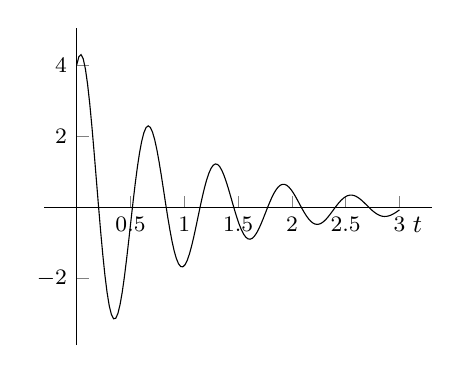
\begin{tikzpicture}
\begin{axis}[small,axis lines*=middle,xlabel={$t$},xlabel style={at={(current axis.right of origin)},anchor=north east}]
\addplot[domain=0:3,samples=150]{e^(-x)*(4*cos(180/pi*10*x)+2*sin(180/pi*10*x))};
\end{axis}
\end{tikzpicture}
\caption{قصری ارتعاش (مثال \حوالہ{مثال_لاپلاس_بدل_قصری_ارتعاش})}
\label{شکل_لاپلاس_قصری_ارتعاش}
\end{figure}
\انتہا{مثال}
%=======================

\جزوحصہء{لاپلاس بدل کی وجودیت اور یکتائی}
اگر تمام  \عددی{t \ge 0} کے لئے، کسی مستقل \عددی{k} اور \عددی{M} پر تفاعل \عددی{f} \موٹا{بڑھنے کی پابندی}
\begin{align}\label{مساوات_لاپلاس_بڑھنے_کی_حد}
\abs{f(t)} \le M e^{kt}
\end{align}
پر پورا اترتا ہو، تب اس کا لاپلاس بدل موجود ہو گا۔ہم کہتے ہیں کہ نہایت تیزی سے نہ بڑھنے والے  تفاعل \عددی{f(t)} کا لاپلاس بدل موجود ہو گا۔

\عددی{f(t)} کا استمراری  ہونا ضروری نہیں ہے البتہ اس کا \اصطلاح{ٹکڑوں میں استمراری}\فرہنگ{استمراری!ٹکڑوں میں}\حاشیہب{piecewise continuous}\فرہنگ{continuous!piecewise} ہونا لازم ہے۔  اگر محدود وقفہ \عددی{a \le t \le b} جس پر \عددی{f(t)} معین ہو، کو کئی ایسے ٹکڑوں میں تقسیم کرنا ممکن ہو کہ ہر ٹکڑے پر \عددی{f(t)} استمراری ہو اور \عددی{t} کا اندرون ٹکڑے سے ٹکڑے کے (دونوں) سروں تک پہنچنے پر  \عددی{f(t)} کی قیمت کا \اصطلاح{حد}\حاشیہب{limit} محدود حاصل ہو تب \عددی{f(t)} \اصطلاح{ٹکڑوں میں استمراری} کہلائے گا۔ ایسی صورت میں، جیسا شکل \حوالہ{شکل_لاپلاس_ٹکڑوں_استمراری} میں دکھایا گیا ہے، محدود \اصطلاح{چھلانگ}\فرہنگ{چھلانگ}\حاشیہب{jumps}\فرہنگ{jumps} پائے جائیں گے جو غیر استمراری صورت کی واحد وجہ ہو گی۔ عموماً عملی مسائل اسی نوعیت کے ہوتے ہیں۔درج ذیل مسئلہ بھی اسی نوعیت کا ہے۔ 
\begin{figure}
\centering
\begin{tikzpicture}
%axis
\draw(0,-1)--(0,2);
\draw(0,0)--++(6,0)node[right]{$t$};
\draw(1,0)--++(0,-0.1)node[below]{$a$};
\draw(5,0)--++(0,-0.1)node[below]{$b$};
%piecewise continuous
\draw(1,0.5) to [out=30,in=-150]++(1,1)node[circ]{};
\draw(2,2) to [out=-20,in=120]++(1,-2.5)node[circ]{};
\draw(3,0.3) to [out=0,in=-145]++(1,0.5)coordinate(kA);
\draw(4,1.4)coordinate(kB)--++(0.4,0)--++(0.6,-0.5);
\draw($(kA)!0.5!(kB)$) node[circ]{};
\end{tikzpicture}
\caption{ٹکڑوں میں استمراری تفاعل \عددی{f(t)}۔ غیر استمراری مقام پر تفاعل کی قیمت کو نقطوں سے ظاہر کیا گیا ہے۔}
\label{شکل_لاپلاس_ٹکڑوں_استمراری}
\end{figure}
%=============

\ابتدا{مسئلہ}\شناخت{مسئلہ_لاپلاس_وجودیت}\quad مسئلہ وجودیت لاپلاس بدل\\
اگر نصف محور \عددی{t \ge 0} کے ہر محدود وقفے پر تفاعل \عددی{f(t)} معین اور ٹکڑوں میں استمراری ہو اور مساوات \حوالہ{مساوات_لاپلاس_بڑھنے_کی_حد} پر، 
تمام \عددی{t \ge 0} اور کسی مستقل \عددی{M} اور \عددی{k} کے لئے،  پورا اترتا ہو تب لاپلاس بدل \عددی{\Laplace (f)} تمام \عددی{s >k} کے لئے موجود ہو گا ۔ 
\انتہا{مسئلہ}
%=========================

\ابتدا{ثبوت}
چونکہ \عددی{f(t)} ٹکڑوں میں استمراری ہے لہٰذا \عددی{t} محور کے کسی بھی محدود وقفے پر \عددی{e^{-st}f(t)} قابل تکمل ہے۔ مساوات \حوالہ{مساوات_لاپلاس_بڑھنے_کی_حد} کو دیکھ کر، \عددی{s>k} تصور کرتے ہوئے (جو درج ذیل آخری تکمل میں درکار ہے)، لاپلاس بدل کی وجودیت کا ثبوت حاصل کرتے ہیں۔
\begin{align*}
\abs{\Laplace(f)} = \abs{\int_{0}^{\infty} e^{-st}f(t)\dif t}\le \int_{0}^{\infty} \abs{f(t)}e^{-st}\dif t\le \int_{0}^{\infty} Me^{kt}e^{-st}\dif t=\frac{M}{s-k}
\end{align*}
\انتہا{ثبوت}
%=========================

کسی بھی تفاعل کا مساوات \حوالہ{مساوات_لاپلاس_بڑھنے_کی_حد} میں دیے گئے شرط پر پورا اترنے کو با آسانی دیکھا جا سکتا ہے، مثلاً \عددی{\cosh t < e^t} یا \عددی{t^n<n!e^t} (چونکہ \عددی{\tfrac{t^n}{n!}} مکلارن تسلسل کا ایک رکن ہے)۔ ایسا تفاعل جو مساوات \حوالہ{مساوات_لاپلاس_بڑھنے_کی_حد} پر پورا نہ اترتا ہو کی مثال \عددی{e^{t^2}} ہے۔آپ سوال \حوالہ{سوال_لاپلاس_کافی} میں دیکھیں گے کہ مسئلہ \حوالہ{مسئلہ_لاپلاس_وجودیت} میں دیے گئے شرائط لاپلاس بدل کی وجودیت کے لئے کافی ہیں نا کہ لازمی ہیں۔

\جزوحصہء{یکتائی}
اگر کسی تفاعل کا لاپلاس بدل موجود ہو تو یہ بدل یکتا ہو گا۔اسی طرح اگر (حقیقی مثبت محور پر معین) دو تفاعل کے لاپلاس بدل یکساں ہوں تب یہ تفاعل، کسی بھی مثبت لمبائی کے وقفے پر،  آپس میں مختلف نہیں ہو سکتے ہیں، البتہ تنہا نقطوں پر ان کی قیمت غیر یکساں ہو سکتی ہے۔یوں ہم کہہ سکتے ہیں کہ الٹ لاپلاس بدل یکتا ہے۔ بالخصوص دو ایسے استمراری تفاعل جن کا لاپلاس بدل یکساں ہو، آپس میں مکمل طور پر یکساں ہوں گے۔ 
%========================

\حصہء{سوالات}
%=============
سوال \حوالہ{سوال_لاپلاس_بدل_الف} تا سوال \حوالہ{سوال_لاپلاس_بدل_ب} میں لاپلاس بدل حاصل کریں۔ \عددی{a} اور  \عددی{b} کو مستقل تصور کریں۔

\ابتدا{سوال}\شناخت{سوال_لاپلاس_بدل_الف}\quad
$2t-3$\\
جواب:\عددی{\tfrac{2}{s^2}-\tfrac{3}{s}}
\انتہا{سوال}
%=======================
\ابتدا{سوال}\quad
$(at+b)^2$\\
جواب:\عددی{a(\tfrac{b}{s^2}+\tfrac{2a}{s^3})+b(\tfrac{b}{s}+\tfrac{a}{s^2})}
\انتہا{سوال}
%=====================
\ابتدا{سوال}\quad
$\sin 2\pi t$\\
جواب:\عددی{\tfrac{2\pi}{s^2+4\pi^2}}
\انتہا{سوال}
%====================
\ابتدا{سوال}\quad
$\sin^2 2\pi t$\\
جواب:\عددی{\tfrac{8\pi^2}{s(s^2+16\pi^2)}}
\انتہا{سوال}
%====================
\ابتدا{سوال}\quad
$e^{-3t}\sin 4t$\\
جواب:\عددی{\tfrac{4}{(s+3)^2+16}}
\انتہا{سوال}
%======================
\ابتدا{سوال}\quad
$e^{2t}\cos 3t$\\
جواب:\عددی{\tfrac{s-2}{(s-2)^2+9}}
\انتہا{سوال}
%======================
\ابتدا{سوال}\quad
$\cos (2t-\frac{\pi}{3})$\\
جواب:\عددی{\tfrac{\tfrac{s}{2}+\sqrt{3}}{s^2+4}}
\انتہا{سوال}
%=========================
\ابتدا{سوال}\شناخت{سوال_لاپلاس_بدل_ب} \quad
$2\sin (5t+\pi)$\\
جواب:\عددی{\tfrac{-10}{s^2+25}}
\انتہا{سوال}
%======================
\begin{figure}
\centering
\begin{subfigure}{0.33\textwidth}
\centering
\begin{tikzpicture}
%axis
\draw[gray](0,0)--(0,1.5);
\draw[gray](0,0)--(3,0);
%function
\draw[thick](0,0)--(2,1);
\draw[dashed](2,1)--(2,0);
\draw[thick](2,0)node[below]{$2$}--(3,0);
\draw(0,1)--++(-0.1,0)node[left]{$1$};
\draw(1,-0.5)node{(الف)};
\end{tikzpicture}%
\end{subfigure}%
\begin{subfigure}{0.33\textwidth}
\centering
\begin{tikzpicture}
%axis
\draw[gray](0,0)--(0,1.5);
\draw[gray](0,0)--(3,0);
%function
\draw[thick](0,1)--(2,1);
\draw[dashed](2,1)--(2,0)node[below]{$3$};
\draw[thick](2,0)--(3,0);
\draw(0,1)--++(-0.1,0)node[left]{$2$};
\draw(1,-0.5)node{(ب)};
\end{tikzpicture}%
\end{subfigure}%
\begin{subfigure}{0.33\textwidth}
\centering
\begin{tikzpicture}
%axis
\draw[gray](0,0)--(0,1.5);
\draw[gray](0,0)--(3,0);
%function
\draw[thick](0,1)--(2,0);
\draw[thick](2,0)node[below]{$5$}--(3,0);
\draw(0,1)--++(-0.1,0)node[left]{$2$};
\draw(1,-0.5)node{(پ)};
\end{tikzpicture}%
\end{subfigure}
%
\begin{subfigure}{0.33\textwidth}
\centering
\begin{tikzpicture}
%axis
\draw[gray](0,-1.2)--(0,1.2);
\draw[gray](0,0)--(3,0);
%function
\draw[thick](0,1)--(2,-1);
\draw[dashed](2,-1)--(2,0);
\draw[thick](2,0)node[above]{$2$}--(3,0);
\draw(0,1)--++(-0.1,0)node[left]{$5$};
\draw(0,-1)--++(-0.1,0)node[left]{$-5$};
\draw(0.75,-0.75)node{(ت)};
\end{tikzpicture}%
\end{subfigure}%
\begin{subfigure}{0.33\textwidth}
\centering
\begin{tikzpicture}
%axis
\draw[gray](0,0)--(0,1.5);
\draw[gray](0,0)--(3,0);
%function
\draw[thick](0,0)--(1,1)--(2.5,0)node[below]{$7$}--(3,0);
\draw(0,1)--++(-0.1,0)node[left]{$2$};
\draw(1,0)--++(0,-0.1)node[below]{$3$};
\draw(1,-0.75)node{(ٹ)};
\end{tikzpicture}%
\end{subfigure}%
\begin{subfigure}{0.33\textwidth}
\centering
\begin{tikzpicture}
%axis
\draw[gray](0,0)--(0,1.5);
\draw[gray](0,0)--(3,0);
%function
\draw[thick](0,0)--(1,1);
\draw[dashed](1,1)--(1,1.5);
\draw[thick](1,1.5)--(2,1.5);
\draw[dashed](2,1.5)--(2,0);
\draw[thick](2,0)node[below]{$4$}--(3,0);
\draw(0,1)--++(-0.1,0)node[left]{$2$};
\draw(0,1.5)--++(-0.1,0)node[left]{$3$};
\draw(1,0)--++(0,-0.1)node[below]{$2$};
\draw(1.5,-0.75)node{(ث)};
\end{tikzpicture}%
\end{subfigure}
\caption{سوال \حوالہ{سوال_لاپلاس_بدل_پ} تا سوال \حوالہ{سوال_لاپلاس_بدل_پ} کے اشکال۔}
\label{شکل_سوال_لاپلاس_بدل_پ}
\end{figure}
%================
\ابتدا{سوال}\شناخت{سوال_لاپلاس_بدل_پ} 
شکل \حوالہ{شکل_سوال_لاپلاس_بدل_پ}-الف میں ٹکڑوں میں استمراری تفاعل دکھایا گیا ہے۔تمام ٹکڑوں کی ریاضی مساوات حاصل کریں۔ تکمل \حوالہ{مساوات_لاپلاس_بدل_الف}  کو ٹکڑوں میں تقسیم کرتے ہوئے لاپلاس بدل حاصل کریں۔

جواب:\عددی{\tfrac{1-e^{-2s}(2s+1)}{2s^2}}
\انتہا{سوال}
%=========================
\ابتدا{سوال}
شکل \حوالہ{شکل_سوال_لاپلاس_بدل_پ}-ب میں دیے گئے تفاعل کا لاپلاس بدل حاصل کریں۔

جواب:\عددی{\tfrac{2}{s}(1-e^{-3s})}
\انتہا{سوال}
%===========================
\ابتدا{سوال}
شکل \حوالہ{شکل_سوال_لاپلاس_بدل_پ}-پ میں دیے گئے تفاعل کا لاپلاس بدل حاصل کریں۔

جواب:\عددی{\tfrac{2e^{-5s}+10s-2}{5s^2}}
\انتہا{سوال}
%===========================
\ابتدا{سوال}
شکل \حوالہ{شکل_سوال_لاپلاس_بدل_پ}-ت میں دیے گئے تفاعل کا لاپلاس بدل حاصل کریں۔

جواب:\عددی{\tfrac{5(s+1)e^{-2s}+5(s-1)}{s^2}}
\انتہا{سوال}
%===========================
\ابتدا{سوال}
شکل \حوالہ{شکل_سوال_لاپلاس_بدل_پ}-ٹ میں دیے گئے تفاعل کا لاپلاس بدل حاصل کریں۔

جواب:\عددی{\tfrac{4-7e^{-3s}+3e^{-7s}}{6s^2}}
\انتہا{سوال}
%===========================
\ابتدا{سوال}
شکل \حوالہ{شکل_سوال_لاپلاس_بدل_پ}-ث میں دیے گئے تفاعل کا لاپلاس بدل حاصل کریں۔

جواب:\عددی{\tfrac{1+(s-1)e^{-2s}-3se^{-4s}}{s^2}}
\انتہا{سوال}
%===========================
\ابتدا{سوال}\شناخت{سوال_لاپلاس_کافی}\quad وجودیت\\
تفاعل \عددی{\tfrac{1}{\sqrt{t}}} کا لاپلاس بدل حاصل کریں۔ایسا کرتے ہوئے \عددی{\Gamma(\tfrac{1}{2})=\sqrt{\pi}} (مساوات \حوالہ{مساوات_بیسل_گیما_نیم}) کا استعمال کریں۔ اس سے آپ اخذ کر سکتے ہیں کہ مسئلہ \حوالہ{مسئلہ_لاپلاس_وجودیت} میں دیے شرائط کافی ہیں نا کہ لازمی۔

جواب:\عددی{\tfrac{\sqrt{\pi}}{s}}
\انتہا{سوال}
%==============================
\ابتدا{سوال}
\عددی{e^{at}} کا لاپلاس بدل \عددی{\cosh at} اور \عددی{\sinh at} کے لاپلاس بدل سے حاصل کریں۔

جواب:\عددی{e^{at}=\sinh at+\cosh at} لکھ کر جواب \عددی{\tfrac{1}{s-a}} ملتا ہے۔
\انتہا{سوال}
%============================
